\documentclass[11pt]{report}
\usepackage[french]{babel}
\usepackage[utf8]{inputenc}
\usepackage[T1]{fontenc}
\usepackage[top = 2cm, bottom = 2cm, left = 2cm, right = 2cm]{geometry}
\usepackage{graphicx}
\usepackage{times}
\usepackage{parskip}
\usepackage{amsfonts}
\usepackage{graphicx}
\usepackage{cprotect}
\usepackage{fancyvrb}

\title{Rapport projet IA04 ~\\ Flotte de drones en 2D}
\author
{
	Mohamed \bsc{Baaziz} ~\\ 
	Lucas \bsc{Sorin} ~\\ 
	Gustavo \bsc{Cabrera} ~\\ 
	Hachem \bsc{Benyahia}
}
\date{13 juin 2016}

\renewcommand{\thesection}{\arabic{section}}

\begin{document}

\maketitle
\renewcommand{\contentsname}{\centering Sommaire \vspace*{1cm}}
\tableofcontents

\newpage

\section{Introduction}

Dans le cadre de l'UV IA04, nous devons réaliser un SMA (\textit{Système Multi-Agents}) évolué à l'aide de la librairie JADE sous Java. L'objectif est donc donc un premier temps de trouver un fonctionnement ou un phénomène modélisable sous le paradigme multi-agents, et implémentable sous JADE, puis précisément de le coder pour ensuite pouvoir le simuler informatiquement. On peut par exemple penser à beaucoup d'exemples connus dans le domaine de l'intelligence artificielle comme le modèle proie-prédateur, l'évolution d'une population d'insectes, le comportement d'une foule, etc. 

Dans la première partie, celle qui suit cette introduction, nous allons décrire le système réel choisi à modéliser. Puis nous verrons les préférences technologiques vers lesquelles nous nous sommes tournés pour l'implémentation. Ensuite une partie pour décrire l'architecture du système conçu. Pour terminer quelques pistes d'amélioration et enfin la conclusion sur ce projet.

\section{Contexte}

Dans cette section, nous allons décrire le projet, en quoi il consiste, son but, son utilité, ses implications dans le monde réel, le contexte global dans lequel il se situe (en dehors de l'UV IA04) ainsi que sa faisabilité.

\subsection{Description du projet}

Comme le titre du rapport l'indique, notre choix s'est porté sur les drones, appareils sur lesquels il y a encore beaucoup à faire et dont les applications sont multiples. Ces appareils sont chers à fabriquer, et lorsque par exemple l'un d'entre eux tombe en panne, surtout s'il est isolé, on peut le considérer comme étant perdu (financièrement parlant). Le fait d'en avoir plusieurs qui se déplacent en flotte a beaucoup d'avantages, l'un d'entre eux étant par exemple que les autres drones, avertis de la chute (sur le sol) de l'un des leurs, pourraient le rapatrier (à la base, dans un contexte militaire typiquement) et le faire réparer par des opérateurs, voire le réparer eux-mêmes (flottes autonomes).

Ceci n'est bien sûr qu'une application possible, et en pratique les flottes de drones peuvent être vues comme un réseau de drones interconnectés et communiquant entre eux afin d'atteindre un objectif donné (qui peut être se déplacer à un endroit, réguler le trafic aérien en optimisant leur déplacement dans le ciel - cas utile s'il y a plusieurs appareils volants dans l'espace en question - etc.).

On voit en quoi les drones sont adaptés au paradigme SMA, chaque drone pouvant être vu comme un agent. Bien sûr, on peut pousser le concept et donner une intelligence artificielle à chaque flotte, ainsi que permettre aux flottes de communiquer sur de très longues distances. En extrapolant, on peut même aller au-delà des drones et suggérer un système autonome d'auto-régulation de tout le trafic (routier, aérien, maritime, etc). Mais pour le projet, ce qui nous intéresse c'est uniquement la simulation d'une flotte de drones, de sa création, à éventuellement sa destruction, en passant par sa fusion avec une autre flotte.

\subsection{Contraintes}

Comme ce projet d'IA04 est limité en temps et en main-d'oeuvre, il faut restreindre le cadre et spécifier les fonctionnalités que nous avons l'intention d'implémenter. En l'occurrence nous allons décrire notre cadre de conception dans la prochaine sous-partie.

\subsubsection{Modélisation} 

On suppose qu'un agent représente un drone et on se place dans un plan 2D ($xOy$). Chaque drone est assimilé à un point qui représente sa position $(x, y)$ dans le plan. La taille du point n'est pas forcément d'un pixel (on pourrait difficilement le voir dans ce cas ...). L'objectif est de faire en sorte que les agents coexistent dans un périmètre donné, leur coexistence devant amener à la formation de flottes (but du projet). Les coordonnées sont positives, on se place dans $\mathbb{R}^{2}_{+}$. L'espace de déplacement (l'environnement) n'est pas torique et est limité par des bornes en $x$ et $y$. L'espace est carré.

\subsubsection{Comportement des drones}

La coexistence des drones est basée sur plusieurs règles de fonctionnement : 

\begin{itemize}
\item Les drones ont tendance à s'organiser en flotte, le nombre de drones maximal dans une flotte est une constante définie au début du programme.

~\
\item Les drones sont démarrés seuls au départ et ne font pas partie d'une flotte.

~\
\item Chaque drone a un unique identifiant.

~\
\item Chaque flotte a un un maître qui guide sa flotte.

~\
\item Les flottes sont en anneau, le diamètre varie en fonction du nombre de drones dans la flotte.

~\
\item La communication des drones se fait par messages à courte portée, ce qui concrètement veut dire qu'un drone ne peut émettre qu'à un certain rayon autour de lui, et de même ne recevoir qu'à une distance inférieure ou égale à ce rayon (en pratique nous avons fait en sorte que chaque drone émette à tous les autres drones mais que les messages soient filtrés en fonction de la distance à l'émetteur).

~\
\item Lorsqu'un drone (ou une flotte) rencontre un autre drone (ou une autre flotte), une procédure est activée de manière à ce que les deux ensembles fusionnent (ou non, en fonction du nombre de drones déjà présents dans la flotte).

~\
\item Lorsqu'un drone est détruit, il est retiré de la liste des drones existants.

~\
\item La communication utilisée dans une flotte est une communication de proche en proche (communication en anneau).
\end{itemize}

\section{Choix technologiques}

Pour concevoir ce système, nous avons fait quelques choix en terme de technologies. Bien sûr, la contrainte du projet est la librairie JADE. Mais il y a également d'autres points à préciser.

\subsection{Interface graphique}

Pour afficher les drones, nous avons utilisé une interface graphique. Cette partie était facultative, mais il aurait été difficile de visualiser leur déplacement dans une console, et donc une GUI (\textit{Graphical User Interface}) semblait particulièrement adaptée à ce cas de figure.

Le rendu visuel est quelque chose comme ceci par exemple (captures faites en cours de développement, on ne voit pas de flottes en anneau, mais certains drones se sont rejoints et se suivent comme on peut le voir de la première capture à la deuxième) :

\begin{figure}[h]
\centering
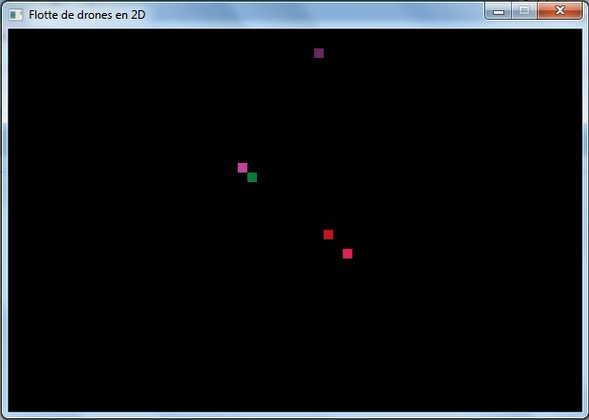
\includegraphics[scale = 0.9]{img/flotte-1.png}
\caption{5 drones sont en train de déplacer (librairie libsdl)}
\end{figure}

\begin{figure}
\centering
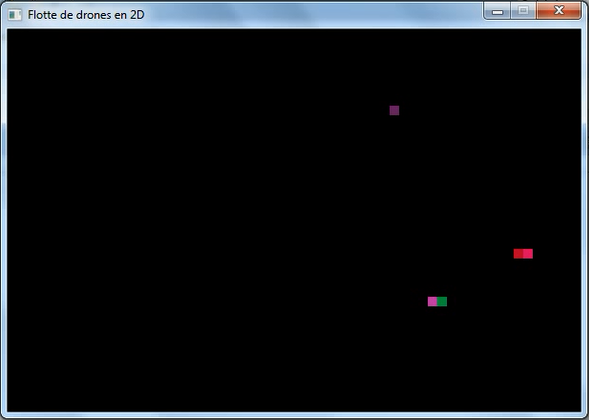
\includegraphics[scale = 0.9]{img/flotte-2.png}
\caption{Les drones se déplacent encore (librairie libsdl)}
\end{figure}

\clearpage

\subsubsection{sdljava (ou libsdl)}

Pour cette interface graphique, nous avons utilisé la librairie \textbf{sdljava}, qui est un \textit{binding} de la librairie \textbf{SDL} du langage C pour le langage Java. Cette librairie est particulièrement adaptée grâce à sa légèreté (une classe suffit à générer la fenêtre graphique).

\subsection{Communication}

La communication des agents Jade (les drones) utilisés dans ce projet se fait en JSON.

\section{Architecture}

Nous allons à présent décrire l'architecture du projet.

L'architecture se divise en trois parties : les drones qui évoluent dans l'environnement 2D, les objets qui se trouvent sur le terrain (partie qui n'a a priori pas été implémentée), et l'interface graphique qui va représenter tout cela sur l'écran. Ces trois parties sont plus ou moins indépendantes. A cela s'ajoutent certaines classes utilitaires et fichiers de constantes. 

Nous n'allons dans ce rapport décrire que ces trois segments, car les autres éléments sont moins pertinents pour l'objet de ce rapport, l'objectif de cette partie étant surtout d'avoir une vue globale du fonctionnement du programme.

\subsection{La classe \protect\Verb+Drone+}

\subsubsection{Description}

La classe \verb|Drone| est la principale classe du projet. En termes de cardinalité, le nombre d'instances de cette classe peut varier de $1$ à $n$.

\subsubsection{Attributs}

Quelques attributs en vrac de la classe \verb|Drone| :

\begin{enumerate}
\item La position actuelle du drone dans le plan $p = (x, y)$ qui est représentée la classe \verb|Position|, qui définit un certain nombre de méthodes (par exemple renvoyer la distance entre deux points du plan).

\item Un identifiant unique.

\item Un état qui indique sa disponibilité (s'il est dans une flotte ou seul par exemple, s'il est actuellement en train de s'intégrer à une flotte existante, etc.).

\item La position objectif du drone (le drone a un objectif par défaut qu'il veut atteindre quand il n'est pas sous la tutelle d'une flotte).

\item Le maitre de sa flotte, s'il appartient à une flotte.

\item Son rang dans la flotte et le voisin auquel il doit envoyer un message (anneau unidirectionnel), s'il appartient à une flotte.
\end{enumerate}

\subsubsection{Behaviours} 

Le drone réagit à son environnement de plusieurs manières, dépendamment des stimuli qui lui parviennent. 

Voici quelques behaviours de la classe \verb|Drone| :

\begin{enumerate}
\item Un behaviour qui renvoie la position de l'agent à l'agent \verb|Display| (que nous allons introduire plus loin) quand il le lui demande.

\item Un behaviour qui envoie spontanément un message à l'agent \verb|Display| lors de la mort de l'agent (l'agent \verb|Display| doit dans ce cas supprimer le drone de la liste des drones et mettre à jour l'affichage).

\item Un behaviour qui réagit aux messages provenant de d'autres éléments de la classe \verb|Drone|.

\item Un behaviour qui envoie périodiquement des messages dans l'environnement immédiat de l'agent (il se contente d'émettre aux autres agents, la réception du message se fait par une fonction de filtration sur l'attribut représentant la position).

\item Un behaviour qui réagit aux messages provenant des objets (dans cette modélisation, les objets sont des ensembles de points fixes dont les points périphériques envoient périodiquement des messages aux drones). Ce behaviour n'a a priori pas été implémenté au regard du manque de temps pour ce projet.
\end{enumerate}

\subsection{La classe \protect\Verb+Display+}

\subsubsection{Description}

La classe \verb|Display| est une classe indépendante de la classe \verb|Drone|. Son rôle est de rapatrier les positions des drones et de les afficher sur une interface graphique. L'implémentation de cette classe passe donc par l'utilisation de sdljava. 

En termes de cardinalité, le nombre d'instances de cette classe est exactement de $1$. C'est la première classe créée lors du lancement du programme, et elle crée les autres objets dès son démarrage. Elle initialise les position des drones (qui peuvent éventuellement être passées en paramètres dans une implémentation plus poussée) et des objets.

\subsubsection{Attributs}

Quelques attributs en vrac de la classe \verb|Display| :

\begin{enumerate}
\item Un tableau dynamique (du fait de la suppression possible de drones au cours de l'évolution de la simulation) recensant les drones existants et leurs positions.

\item Le nombre de drones existants.

\item Un tableau dynamique recensant les objets sur le terrain (si cela est implémenté).

\item Le nombre d'objets existants (idem).
\end{enumerate}

\subsubsection{Behaviours}

Voici quelques behaviours de la classe \verb|Display| :

\begin{enumerate}
\item Un behaviour qui envoie périodiquement à tous les agents \verb|Drone| une demande de leur position. Il met à jour le tableau de positions.

\item Un behaviour qui reçoit un signal de mort de la part d'une drone, dans ce cas il devra le supprimer de sa liste de drones.

\item Un behaviour qui répond un signal d'arrêt en provenance de la console, il supprimera tous les drones et objets et terminera l'exécution (cela n'a a priori pas été implémenté).
\end{enumerate}

\subsection{La classe \protect\Verb+Object+}
\subsubsection{Description}

La classe \verb|Object| n'a pas été implémentée (il me semble). Elle représente les objets qui se trouvent sur le terrain. Les objets sont des polygones. Un objet est un ensemble de points dont les points frontaliers sont ceux qui émettent des messages (il est important de rappeler que les points ne sont pas des pixels, mais des surfaces carrées d'une certaine dimension).

\subsubsection{Attributs}

Quelques attributs en vrac de la classe \verb|Object| :

\begin{enumerate}
\item Un tableau de points représentant la totalité des points qui le composent.

\item Un identifiant unique.
\end{enumerate}

\subsubsection{Behaviours}

Voici quelques behaviours de la classe \verb|Object| :

\begin{enumerate}
\item Un behaviour qui émet constamment des messages (destinés aux agents) dans les environs de l'objet. Seuls les points frontaliers doivent émettre des messages.

\item Un behaviour qui renvoie l'ensemble des points le constituant à l'agent \verb|Display| lorsqu'il le lui demande.
\end{enumerate}

\subsection{La classe \protect\Verb+GUI+}
\subsubsection{Description}

La classe \verb|GUI| est la classe représentant l'interface graphique. Son intégration dans le SMA décrit précédemment a été particulièrement épineuse par construction de son fonctionnement. En effet, comme cette classe contient un \textit{while} qui s'exécute en permanence dans l'attente d'évènement provenant de la GUI, son instanciation bloque le code. De telle sorte que pour qu'elle libère la JVM et que les autres agents puissent s'exécuter également, il a fallu en faire un agent. De manière à ce qu'elle se \textit{détache} de la classe appelante (celle qui l'instancie). Cependant, comme son constructeur est toujours basé sur un \textit{while}, ce n'est qu'un agent sur la forme, et donc elle ne possède pas de behaviours.

Pour rafraîchir l'interface, elle appelle périodiquement une méthode qui dispose d'une \textit{référence} sur l'agent \verb|Display| afin d'acquérir des informations sur l'état actuel des drones. De tel sorte que bien que cette classe soit un agent, \textbf{elle ne communique pas par messages}.

\subsubsection{Attributs}

Quelques attributs en vrac de la classe \verb|Object| :

\begin{enumerate}
\item Une référence sur l'agent \verb|Display|.

\item Un tableau de surfaces (concept de la librairie sdljava) représentant chaque drone et sa couleur.

\item Une référence sur l'écran actuel (la GUI), ce qui est également lié à sdljava.
\end{enumerate}

\section{Pistes d'amélioration}

\section{Conclusion}

\end{document}